\subsubsection{Descripción y grafo de relación entre los nodos}

Nuestro segundo experimento consistió en capturar los paquetes de la LAN Wi-Fi de la empresa Honeywell. En esta red no hay mucho tráfico, ya que la mayoría de las computadores se conectan via Ethernet a una VPN. Esta red es dedicada a transacciones que no necesiten un nivel de seguridad (para uso de teléfonos celulares más que nada). La captura se realizo un día lunes a las 11 am. durante media hora, lográndose capturar 253 paquetes.  

\begin{figure}[H]
 \begin{center}
  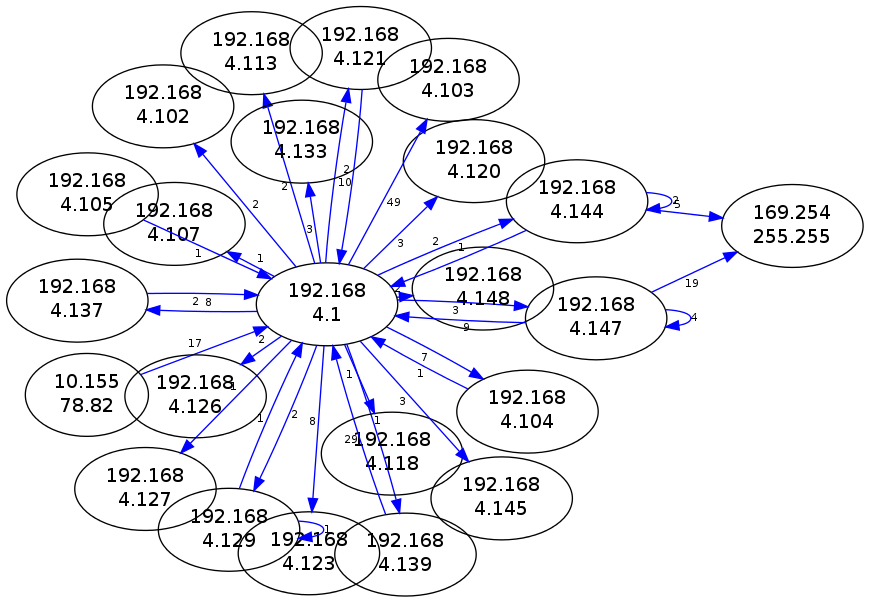
\includegraphics[width=0.7\linewidth]{../imgs/red-honeywell_red.png}
  \caption{Medición Honeywell}
 \end{center}
\end{figure}

El primer nodo que se destaca a simple vista es el \emph{192.168.4.1}, que es el \emph{src} o \emph{dst} de casi todo paquete encontrado.
También distinguimos \emph{169.254.255.255} ya que es el único nodo que no es vecino de \emph{192.168.4.1}.

\subsubsection{Fuente: $S_{dst}$}

\begin{figure}[H]\centering
    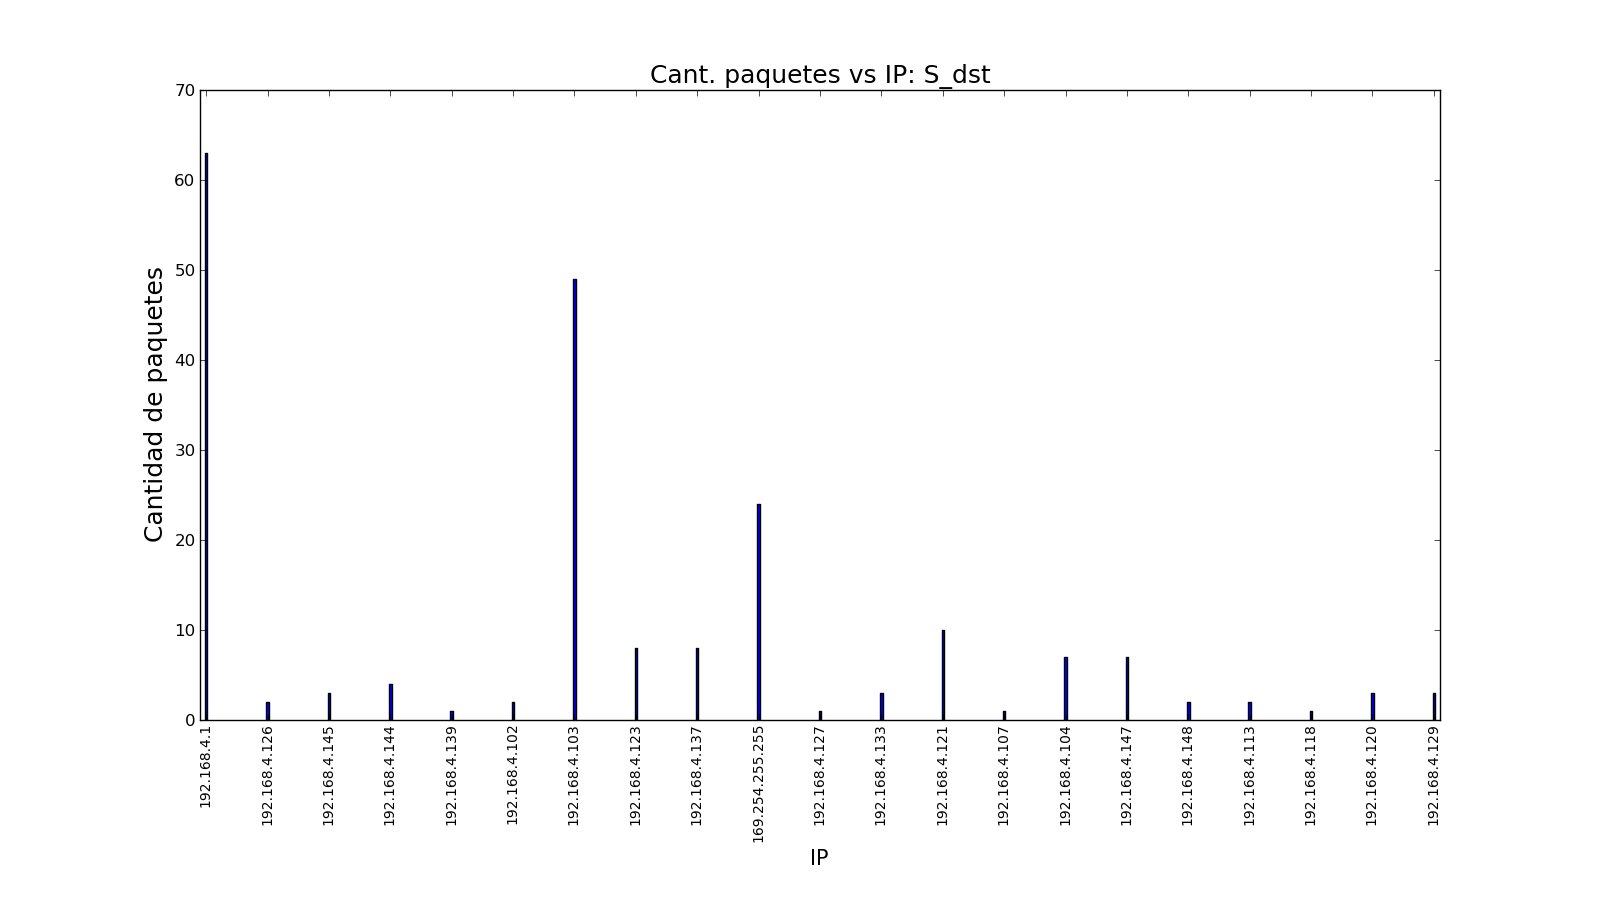
\includegraphics[width=0.8\linewidth]{../imgs/red-honeywell_S_dst_hist.png}
    \caption{Histograma de $S_{dst}$}\label{fig:Honeywell-dst-hist}
\end{figure}

\begin{figure}[H]\centering
    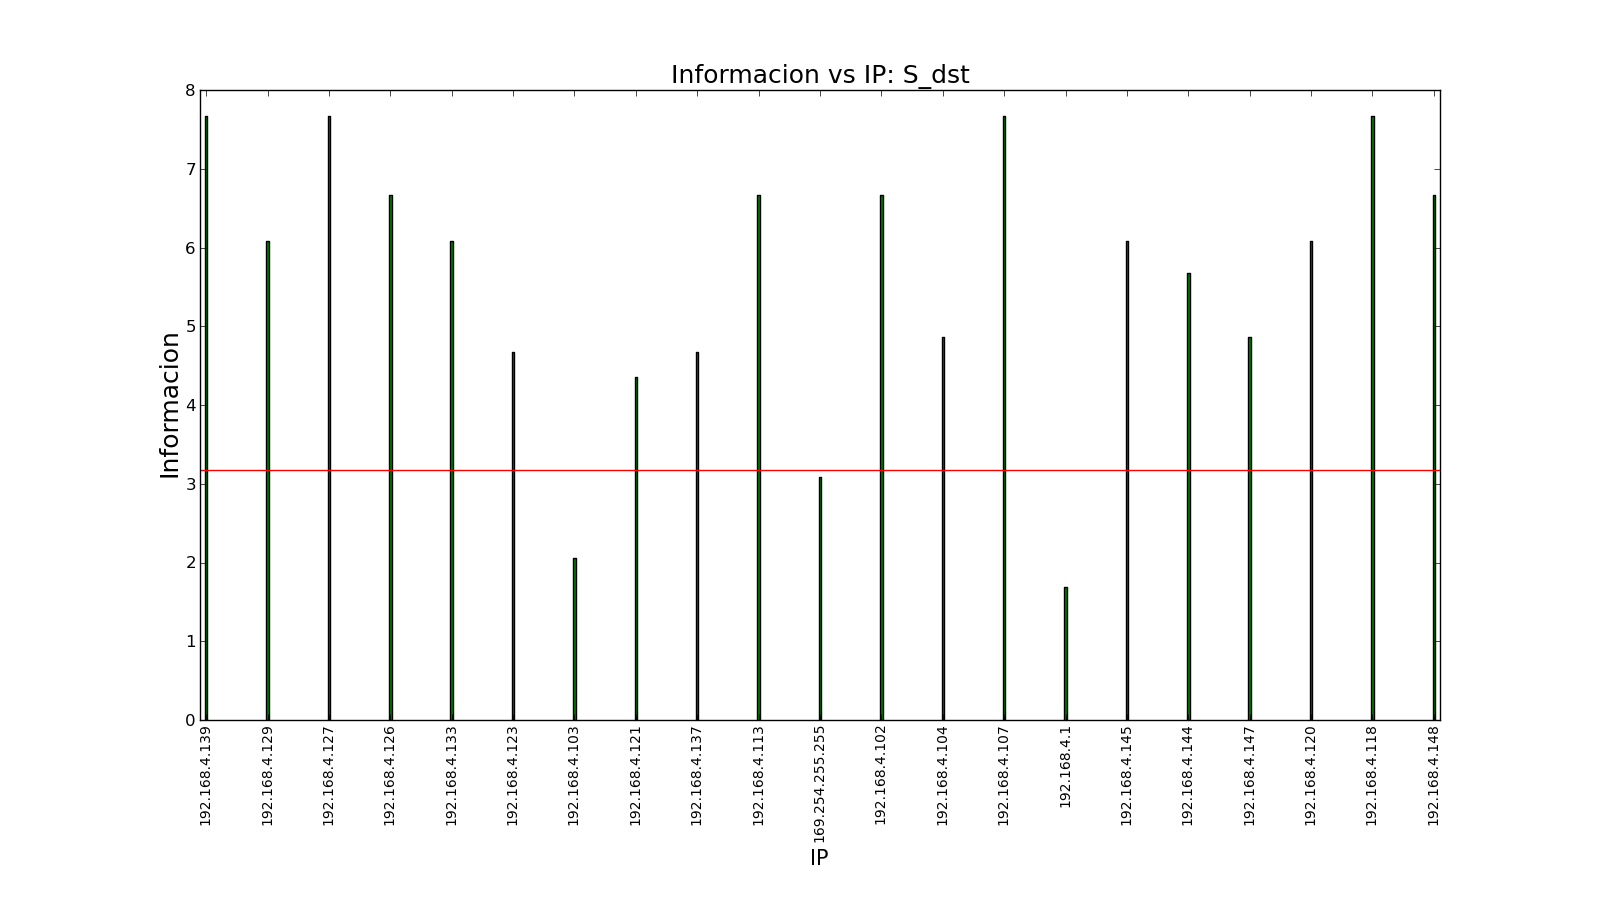
\includegraphics[width=0.8\linewidth]{../imgs/red-honeywell_S_dst_info.png}
    \caption{Informacion de $S_{dst}$}\label{fig:Honeywell-dst-info}
\end{figure}
En la Figura \ref{fig:Honeywell-dst-hist} podemos ver 3 nodos visualmente distinguibles, \emph{192.168.4.1}, \emph{192.168.4.103} y \emph{169.254.255.255}.
Cuando analizamos la Figura \ref{fig:Honeywell-dst-info}, podemos corroborar que estos nodos son distinguidos, ya que su información es menor a la entropía de la fuente.

$\bullet$ Entropía de la fuente: 3.17600221734

\subsubsection{Fuente: $S_{src}$}

\begin{figure}[H]\centering
    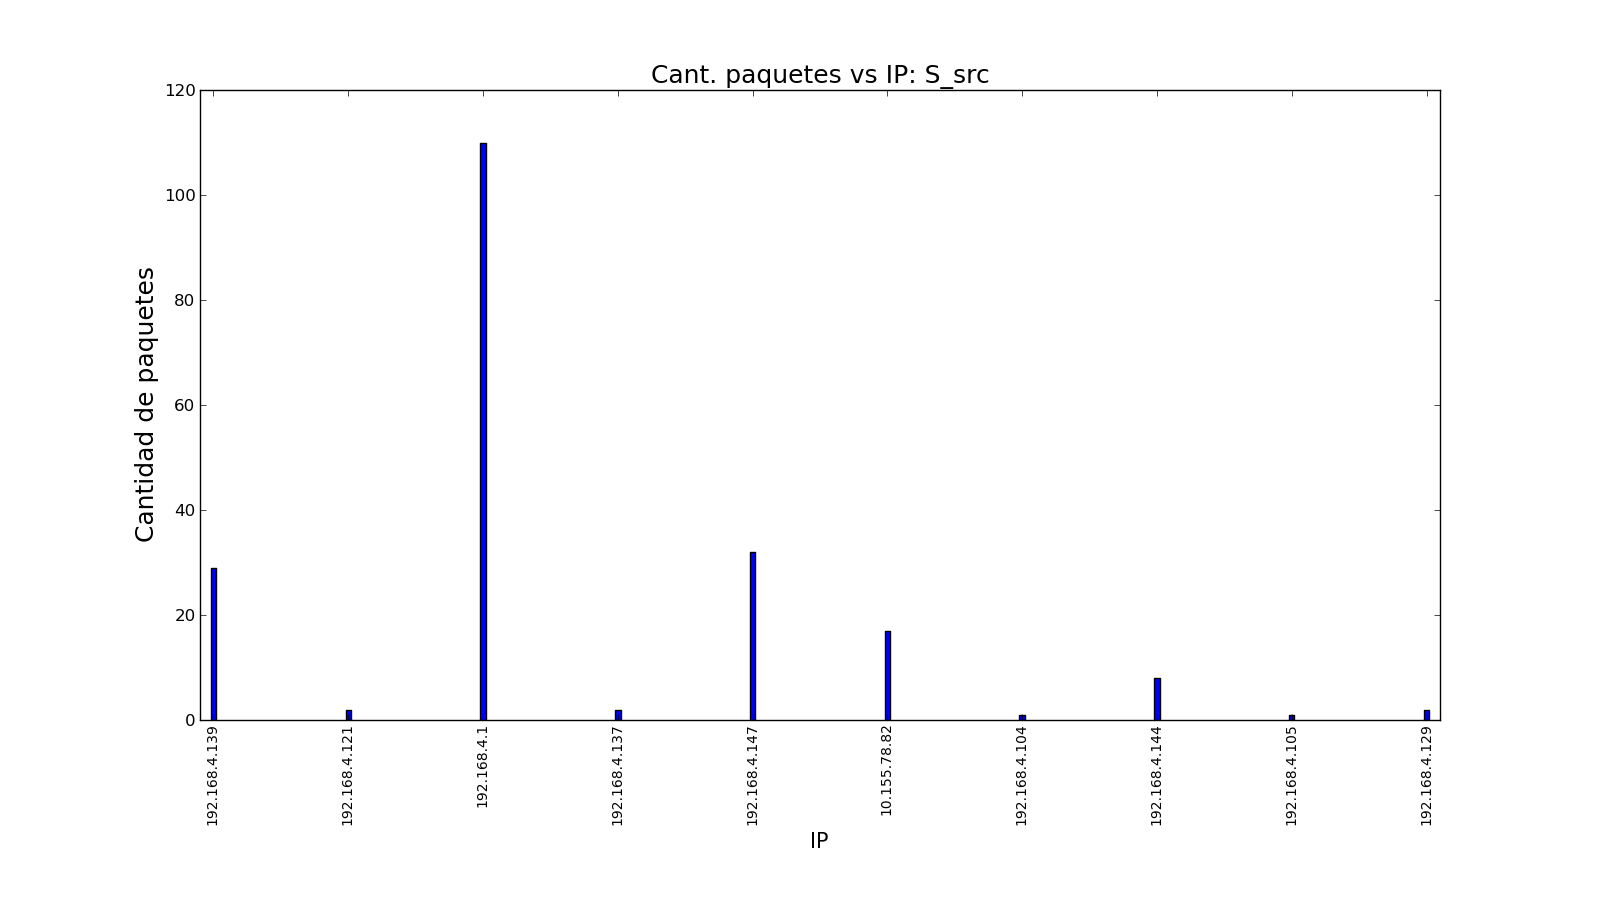
\includegraphics[width=0.8\linewidth]{../imgs/red-honeywell_S_src_hist.png}
    \caption{Histograma de $S_{src}$}\label{fig:Honeywell-src-hist}
\end{figure}

\begin{figure}[H]\centering
    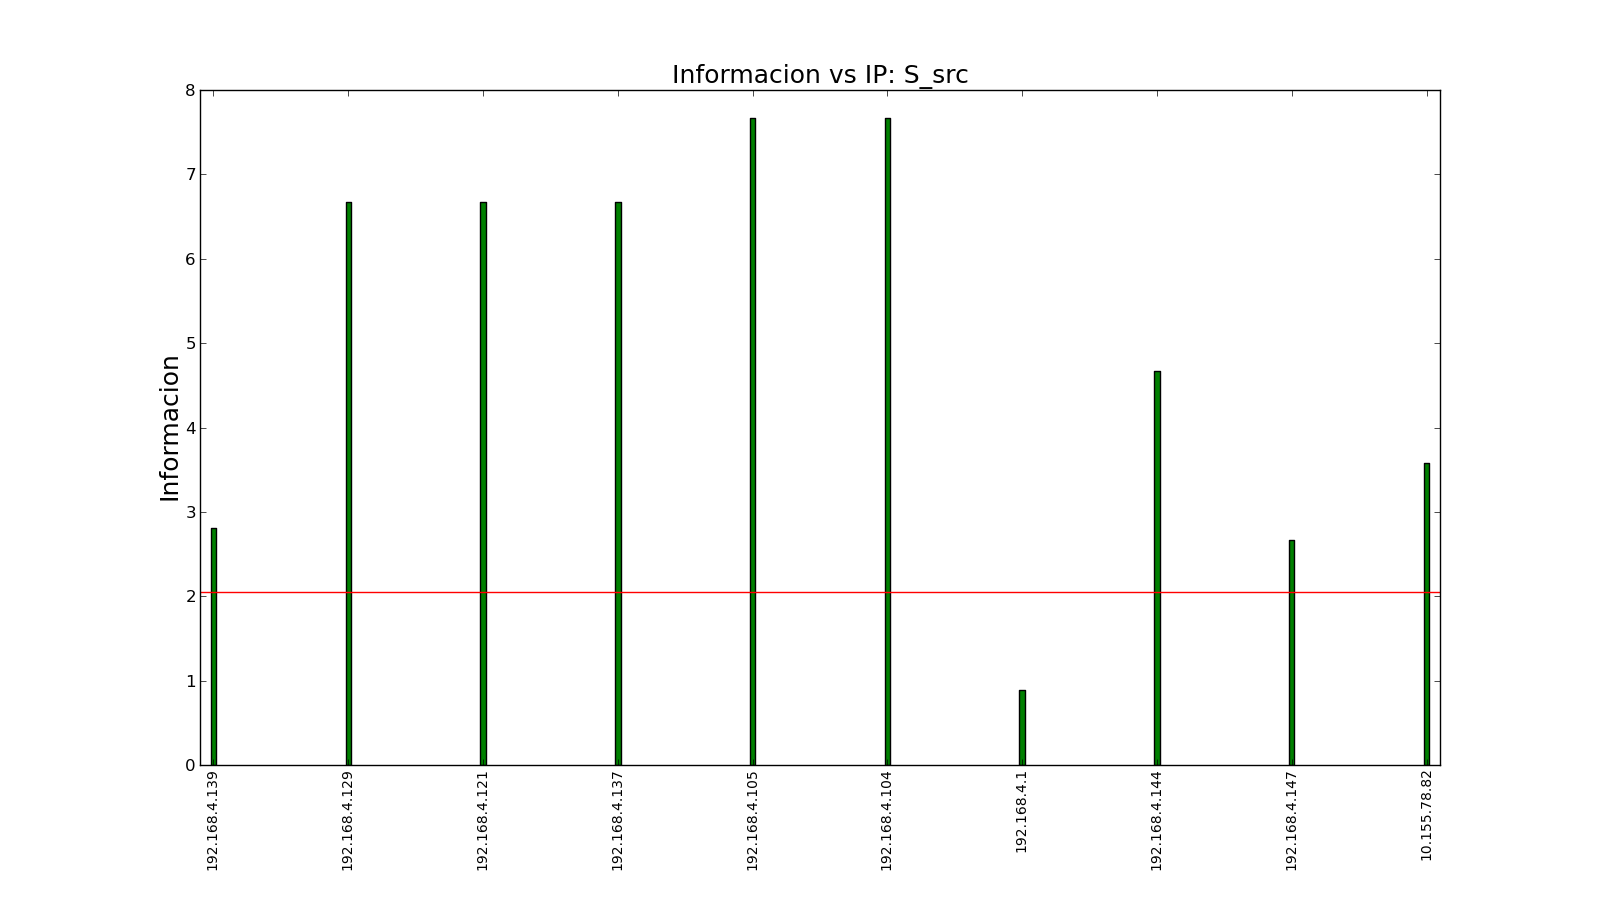
\includegraphics[width=0.8\linewidth]{../imgs/red-honeywell_S_src_info.png}
    \caption{Informacion de $S_{src}$}\label{fig:Honeywell-src-info}
\end{figure}

En la Figura \ref{fig:Honeywell-src-hist} podemos ver un nodo visualmente distinguible, \emph{192.168.4.1}.
Cuando analizamos la Figura \ref{fig:Honeywell-src-info}, podemos corroborar que este nodo es distinguido, ya que su información es menor a la entropía de la fuente.

$\bullet$ Entropía de la fuente: 2.05322002017

\subsubsection{Discusión}

Suponemos que \emph{192.168.4.1} es el router de la red, ya que no solo es un nodo distinguido, sino que vemos en la red que tiene transacciones con casi todos los nodos de la red.
Suponemos que \emph{169.254.255.255} suponemos que es una dirección de \emph{broadcast}, ya que no solo termina con 255.255 (dieciséis 1 en binario), sino que además tiene alta probabilidad como \emph{dst} pero nunca aparece como \emph{src}.
Suponemos que \emph{192.168.4.103} es una terminal con un alto acceso a internet en el momento de la medición (descarga), ya que es un nodo destacado como \emph{dst}, pero no aparece como \emph{src}. Y todos la paquetes los recibe de \emph{192.168.4.1} (que supusimos es el router). 